
\subsubsection{Loss Distribution Separation}

At epoch 5, minority and majority samples exhibit substantially different loss distributions:

\begin{table}[htbp]
\centering
\resizebox{\columnwidth}{!}{%
\begin{tabular}{llll}
\toprule
Statistic & Minority & Majority & Ratio \\
\midrule
Mean loss & 0.158 & 0.019 & 8.$3\times$ \\
Median loss & 0.057 & 0.001 & $57\times$ \\
\bottomrule
\end{tabular}
}
\end{table}

The Mann-Whitney U test confirms statistical significance: U = 705,391, p = 7.36 $\times 10^{-15}$.

\begin{figure}[htbp]
\centering
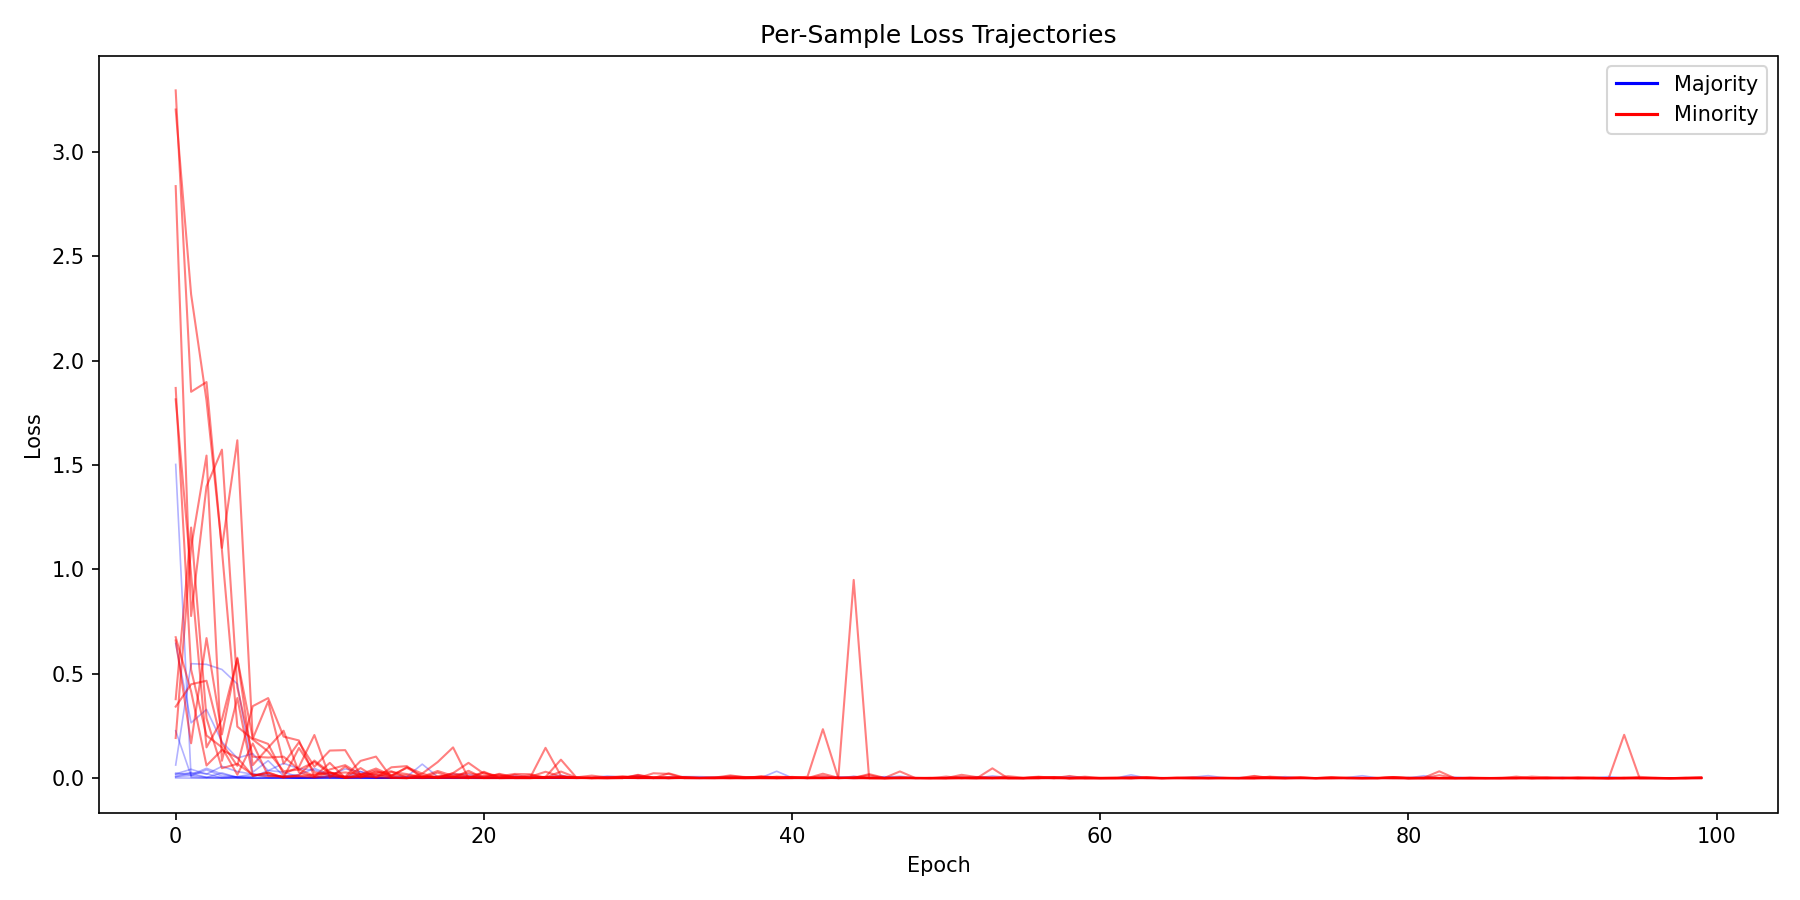
\includegraphics[width=\columnwidth]{figures/loss_trajectories.png}
\caption{Loss trajectories by group}
\label{fig:loss_trajectories}
\end{figure}

\textit{Figure 1: Per-sample loss trajectories colored by group membership. Minority samples cluster in the high-loss region throughout training.}

\subsubsection{Detection Performance}

Using the 95th percentile loss threshold at epoch 5:

\begin{table}[htbp]
\centering
\resizebox{\columnwidth}{!}{%
\begin{tabular}{llll}
\toprule
Metric & Value & Random Baseline & Lift \\
\midrule
Precision & 0.329 & 0.050 & 6.$6\times$ \\
Recall & 0.329 & 0.050 & 6.$6\times$ \\
\bottomrule
\end{tabular}
}
\end{table}

The 6.$6\times$ lift over random demonstrates substantial detection signal. The precision value of 32.9\% approaches the theoretical maximum achievable when predicting 5\% of samples at a 5\% minority base rate---approximately 33\%---indicating that the ranking performance is near-optimal given the base rate constraint.

\begin{figure}[htbp]
\centering
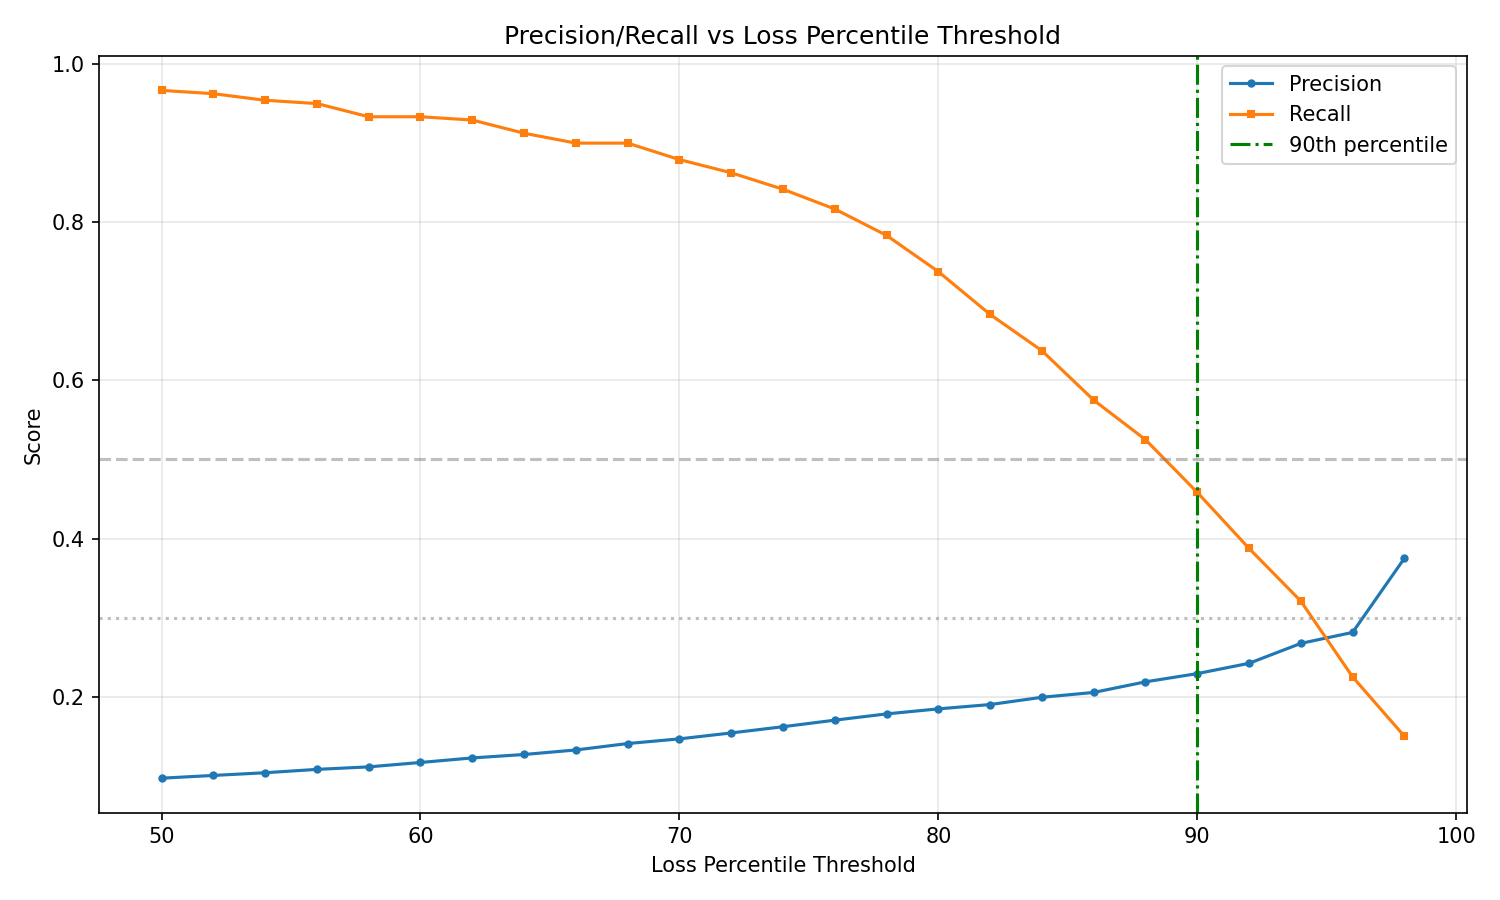
\includegraphics[width=\columnwidth]{figures/pr_curve.png}
\caption{Precision-Recall curve}
\label{fig:pr_curve}
\end{figure}

\textit{Figure 2: Precision-recall curve for minority detection versus loss percentile threshold.}

\subsubsection{Simplicity Bias Mechanism}

Linear probe analysis confirms the presence of simplicity bias:

\begin{table}[htbp]
\centering
\resizebox{\columnwidth}{!}{%
\begin{tabular}{llll}
\toprule
Epoch & Spurious Acc & Core Acc & Gap \\
\midrule
5 & 91.20\% & 80.50\% & +10.70\% \\
20 & 91.59\% & 82.26\% & +9.33\% \\
50 & 91.34\% & 82.62\% & +8.72\% \\
\bottomrule
\end{tabular}
}
\end{table}

At epoch 5, representations encode background information with 91.2\% probe accuracy while bird type achieves 80.5\%---a 10.7 percentage point gap. This gap persists throughout training, confirming that spurious features maintain an encoding advantage.

\begin{figure}[htbp]
\centering
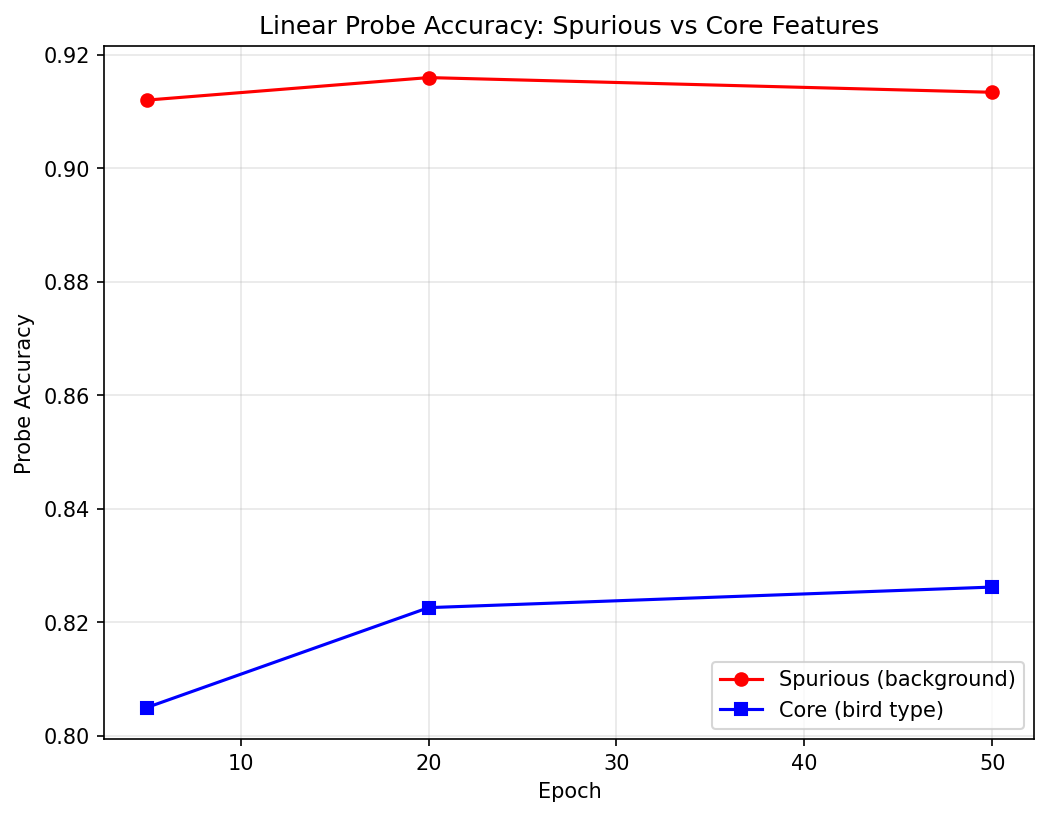
\includegraphics[width=\columnwidth]{figures/probe_accuracy.png}
\caption{Probe accuracy comparison}
\label{fig:probe_accuracy}
\end{figure}

\textit{Figure 3: Linear probe accuracy for spurious (background) versus core (bird type) features across training epochs.}

\subsubsection{Timing Analysis}

The hypothesis that spurious features would peak earlier than core features was not supported. Both feature types reached peak probe accuracy at the same epoch:

\begin{table}[htbp]
\centering
\resizebox{\columnwidth}{!}{%
\begin{tabular}{lll}
\toprule
Feature Type & Peak Epoch & Peak Accuracy \\
\midrule
Spurious & 81 & 91.9\% \\
Core & 81 & 82.8\% \\
\bottomrule
\end{tabular}
}
\end{table}

The Wilcoxon signed-rank test confirms the curves are statistically different (p = 3.88 $\times 10^{-18})$, but this difference manifests as a consistent magnitude gap (~9-11\%) rather than a temporal offset.

\begin{figure}[htbp]
\centering
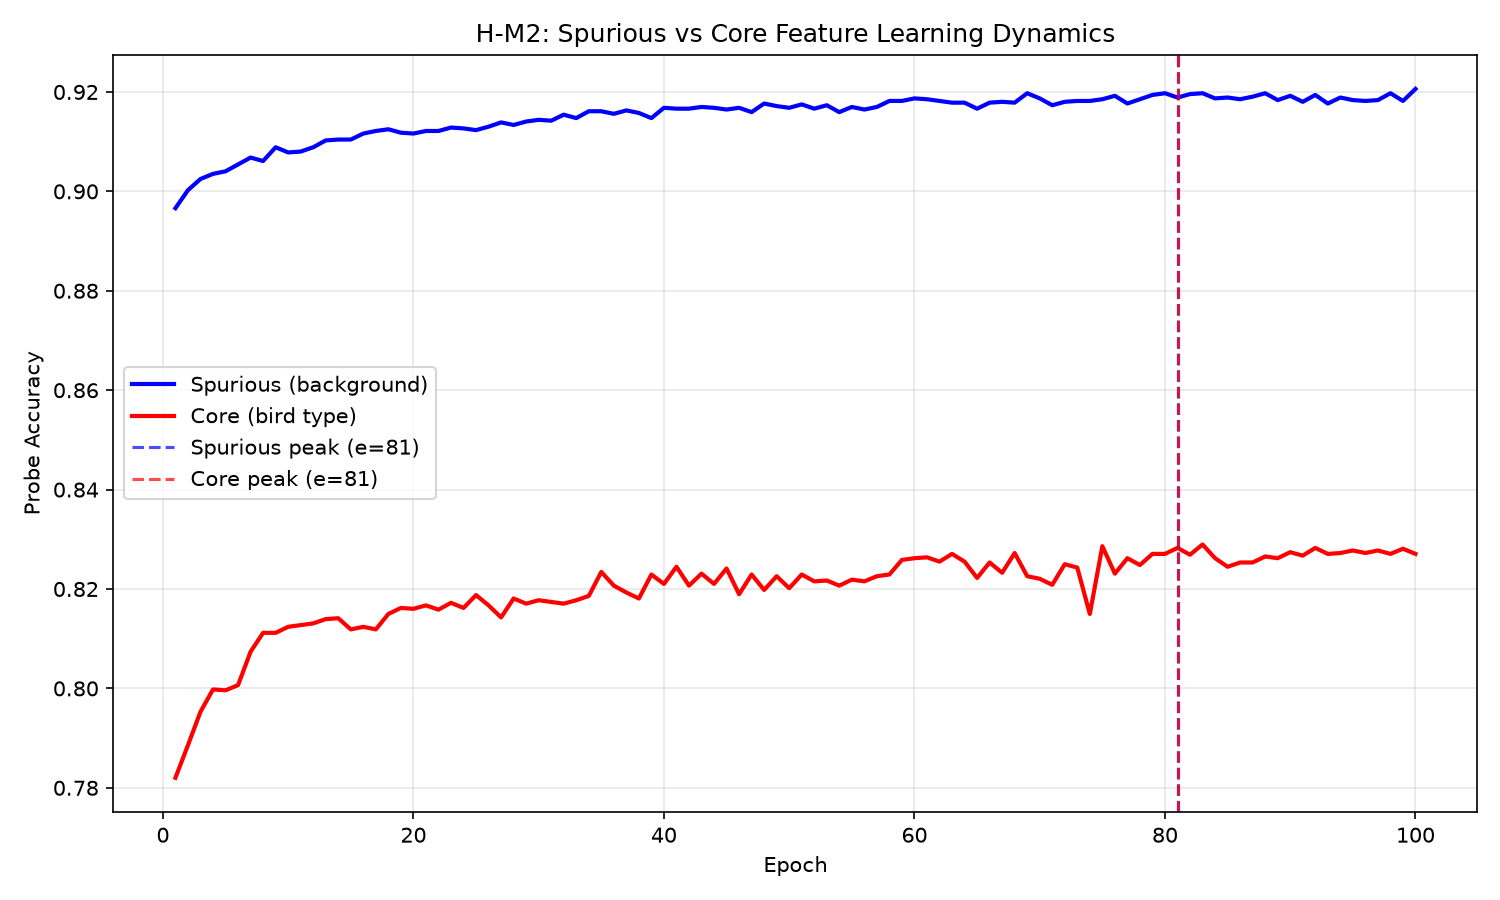
\includegraphics[width=\columnwidth]{figures/learning_curves.png}
\caption{Learning curves}
\label{fig:learning_curves}
\end{figure}

\textit{Figure 4: 100-epoch linear probe learning curves showing parallel trajectories with persistent magnitude gap. Both feature types peak at epoch 81.}

